

This section describes the specific tools used in the experiments and a brief overview of the three test applications. 

%This section describes the specific tools used in the experiments. It starts with presenting the deployed Kubernetes cluster's layout. Then, the tools needed to run the actual experiments are introduced. Finally, this section concludes with a brief overview of the three test applications used.

\paragraph{Kubernetes cluster.}
\label{cluster}
All the experiments are run on a Kubernetes cluster deployed on the DistriNet private cloud, which is based on the OpenStask platform~\citep{openstack}. Four virtual machines are deployed: one master and three worker nodes. The cluster itself is created using \textit{kubeadm}~\citep{kubeadm}. All of the machines are running the Ubuntu 16.04 operating system. Three of the nodes, including the master node, are allocated 2 CPUs and 4 GB of memory. The last node is assigned 4 CPUs and 8 GB of memory. The three worker nodes are placed on the same OpenStack computing node to minimize latencies between applications running on the nodes. On the first worker node, which is the node with 4 CPUs and 8GB of memory, an experiment controller is deployed. The second and third worker nodes are reserved for the applications to be deployed on. An overview of the setup is shown in Figure \ref{fig:cluster}.

\begin{figure}
\centering
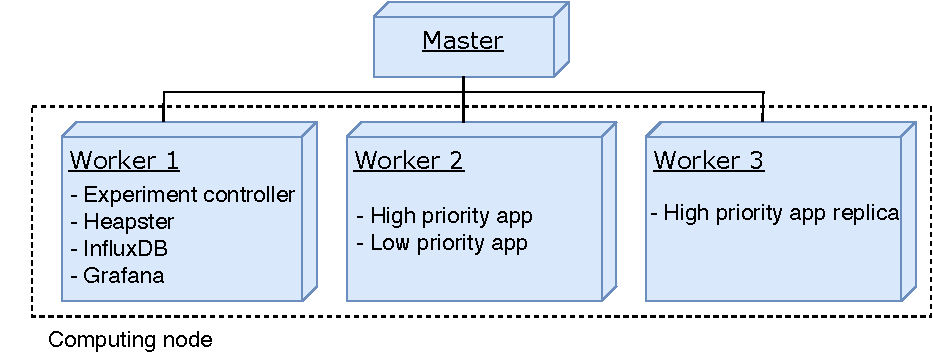
\includegraphics[width=0.85\columnwidth]{Images/Setup/Cluster.pdf}
\caption{Test cluster setup}
\label{fig:cluster} 
\end{figure}


\paragraph{Experimentation tools.}
\label{tools}
%
%\subsubsection{Resource monitoring}
To monitor the resources in the cluster, a combination of Heapster~\citep{heapster}, InfluxDB~\citep{influxdb} and Grafana~\citep{grafana} is employed. To run and monitor the experiments, K8-Scalar~\citep{scalar} is used. K8-Scalar is an extensible workbench exemplar for implementing and evaluating different self-adaptive approaches to autoscaling container-orchestrated services~\citep{scalar-github-overview}.
%Heapster collects each node's metrics through the kubelet node agent~\citep{kubelet}~\citep{heapster-influxdb-grafana}. The collected data is written to InfluxDB. InfluxDB is a time-series database, a database optimized for time-stamped or time series data~\citep{timeseriesdb}. Grafana is a metric dashboard and graph editor which supports, among others, InfluxDB~\citep{grafana-github}. 

%\subsubsection{Experiment controller}
 
%K8-Scalar can be customized to test a specific system by implementing Java user and request classes fit for that system. Multiple users may be implemented, for example one user which performs CPU-intensive requests and one which performs memory-intensive requests. When preparing an experiment, the distribution of the types of users can be specified, for example 95\% of the users executing memory intensive requests and 5\% executing CPU intensive requests. Furthermore, the exact workload profile can be described using a template.
%, part of which is shown in listing \ref{listing:profile}
%An experiment in K8-Scalar consists of multiple runs, and the peak load for each of these runs must be provided. A run in turn consists of a ramp-up phase, a peak load phase and a ramp-down phase. The duration of all of these phases can be configured. In between runs, there can also be constant low load phases. Ramping up and down is done linearly. Besides sending the requests, K8-Scalar monitors the time needed by the tested applications to process these requests~\citep{scalar}.
%
%\lstset{caption={Load profile example},label=listing:profile}
%\begin{lstlisting}[float]
%## LOAD PROFILE
%user_peak_load=500,1000,1500
%user_warmup_fraction=1
%user_warmup_duration=0
%user_ramp_up_duration=0
%user_peak_duration=400
%user_ramp_down_duration=0
%user_cooldown_duration=0
%user_wait_inbetween_runs=0
%\end{lstlisting}
%
\subsection{Deployed applications}
\label{test-apps}

\paragraph{Cassandra based application.}
A Cassandra based application is selected as the first high priority test application. Only write operations are examined in this paper, as they are CPU intensive. The main QoS requirement for the application is thus the latency of write requests. Cassandra is well-suited for the experiments as its design is optimized for write-heavy workloads~\citep{scalar}.

\paragraph{Artificial SaaS application.}
\label{setup:saas-app}
An artificial SaaS application developed at KU Leuven~\citep{saas-app} is selected as a second high priority test application. The main benefit of this SaaS application is that the stressed resource is easily configurable through the application's REST interface. For example, if a CPU intensive workload needs to be tested, the memory intensity of the application can be set to zero by executing a simple REST command at runtime. 

\paragraph{Low priority application.}
\label{setup:lpp}
%The application shown in Figure \ref{fig:cpu-app-python} is deployed as t
The low priority application used for testing the effects of co-locating pods executes a multiplication in an infinite loop. If sufficient resources are free, it continually uses a full CPU since it is single threaded. The exact CPU usage is known and roughly constant.
